\documentclass{article}
\usepackage{graphicx}
\usepackage[margin=1.5cm]{geometry}
\usepackage{amsmath}
\usepackage{hyperref}

\begin{document}
\twocolumn

\title{PhET/Lab Activity: Work and Energy with Springs}
\author{Prof. Jordan C. Hanson}

\maketitle

\section{Introduction}

Our task is to predict the work required to compress a spring.  This calculation is relevant for a multitude of physical systems that \textit{oscillate.}  The work done by compressing a spring by $\Delta \vec{x}$ is 

\begin{equation}
\Delta W = \vec{F} \cdot \Delta \vec{x}
\end{equation}

The force required by Newton's 3rd law is $\vec{F} = k\Delta \vec{x}$, the opposite of the spring force.  Combining equations, we find

\begin{equation}
\Delta W = k\Delta \vec{x} \cdot \Delta \vec{x} = k (\Delta x)^2 \label{eq:1}
\end{equation}

\textbf{There is one complication:} each time we displace the spring another $\Delta x$, the force changes, so $\Delta W$ changes.  We must \textit{add up} all the contributions $\Delta W$ to obtain the total work done, $W$.

\section{Simulation of Spring Behavior}

Load the following PhET simulation: \url{https://phet.colorado.edu/en/simulations/hookes-law}.  Click on the energy tab.  Click on the Force Plot button, and add the energy by checking the Energy box.  We see a linear plot appear that displays the force on the y-axis and the displacement on the x-axis.

Set the spring constant to 300 N m$^{-1}$, and the displacement to zero.  Fill in Tab. \ref{tab:1} below with each $\Delta x$, the \textit{change} in position, $\Delta W$, the \textit{change} in total energy, and the cumulative value for $W$, assuming $k = 300$ N m$^{-1}$.  The cumulative value $W$ is a sum of all previous $\Delta W$ values.

\begin{table}[hb]
\centering
\begin{tabular}{| c | c | c |}
\hline
$\Delta x$ (cm) & $\Delta W$ (J) & $W$ (J) \\
0.1 & & \\
0.2 & & \\
0.3 & & \\
0.4 & & \\
0.5 & & \\
0.6 & & \\
0.7 & & \\
0.8 & & \\
0.9 & & \\
1.0 & & \\
\hline
\end{tabular}
\caption{\label{tab:1} (Left) Change in position. (Center) Change in work done. (Right) Total work done.}
\end{table}

\section{Analysis of Results}

\textbf{Create a graph of $W$ versus $x$}, that is, a graph of spring position versus cumulative work done.  Now add a quadratic curve of the following form to your graph: $W = \frac{1}{2} k x^2$.  Note that the \textit{area} under the curve is the work done, because for each little change $\Delta x$, we add $\vec{F} \cdot \Delta \vec{x}$ to the total work done.  Can you see why the formula $W = \frac{1}{2} k x^2$ works geometrically, from the graph of Applied Force versus position in the simulation?Consider Fig. \ref{fig:1} (top).  The work done by $F$ is the produce of each little displacement $d$ and the instantaneous value for $F\cos\theta$.  \textbf{Repeat the experiment, but with a real spring, using gravity and weights to control the applied force.  Measure the change in height versus the applied force, and note that the change in potential energy for the weight is $U = mg\Delta y$.} \\ \vspace{5cm}

\begin{figure}[hb]
\centering
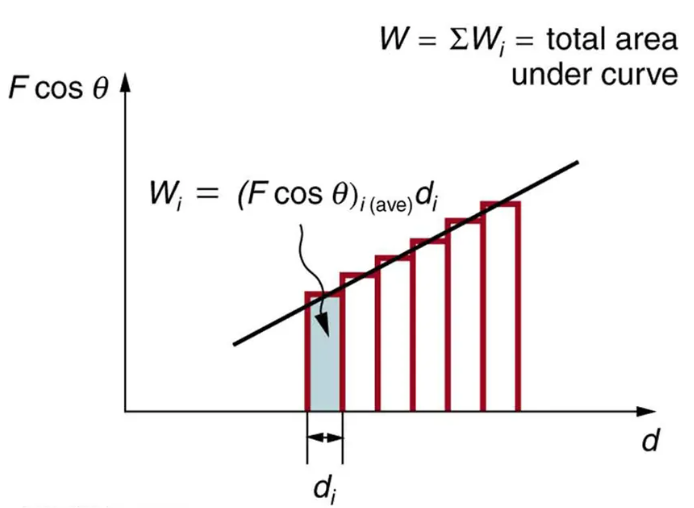
\includegraphics[width=0.45\textwidth]{figures/work_diagram_3.png}
\caption{\label{fig:1} Work done with a linear force.}
\end{figure}

\end{document}
